\section{Design of UV Raman experiment}

Work on the construction of a new UV Raman spectrometer was an incremental
process. It was necessary to consider the equipment already present in the lab,
mainly the laser system, CCD camera and optical table and specify parameters of
chosen commercial spectrograph. Then the first functional prototype was
constructed and improved for measurement of polarized UV Raman spectra. The
first wavenumber calibration technique of measured Raman spectra
was adopted based on the literature. Then we started to deal with
photo-decomposition of samples by designing a spinning cell which could contain
as small as cca. 20 \g{m}l volumes of samples. After that we widened the range
of usable excitation wavelengths of the instrument and decided to seek for a
new means of wavenumber calibration and after some research and trials and
errors we settled with calibration to the spectra of Pt lamp. And then, the
aparatus was enhanced to enable temperature measurements in backscattering
geometry. Next sections describe each step of the development of the UV Raman
spectrometer in more details.


\subsection{Initial equipment}
\label{initial_equipment}

As an excitation source, we used the Coherent Innova 300C
MotoFreD\texttrademark{} Ion Laser which enables intracavity frequency
doubling~\parencite{Asher1993b} of fundamental Ar ion emission lines by
nonlinear crystal. As a frequency doubling crystal we used BBO crystal (also
from Coherent) designed for doubling 488\,nm. Later we extended our
experimental options with additional two crystals designed for doubling 514 and
457\,nm. The BBO crystals are hygroscopic so they needed to be purged by steady
flow of 0.25--0.5 l/min of dry nitrogen of at least grade 5 purity (99.999\%)
\CITATION(laser manual). As a source of this nitrogen we decided to use
nitrogen generator NG1/1 from Gas Generation LTD which uses the pressure
swing absorption technology.

The above mentioned crystals could be used for
frequency doubling also the adjacent Ar ion lines. All the frequency doubled
wavelengths and expected and measured output laser beam powers which we could
tune with these three crystals are listed in
\tabref{initial_equipment:laser_power_spec}. The output wavelengths were
measured with HighFinesse High Precision Wavelength Meter WS5 UV-II and output
powers were measured with Power Meter from Thorlabs. The output powers in the
table were somewhat maximal which we could achieve, usually the power was
lower depending on laser condition. The 264.342\,nm wavelength was not possible
with our laser configuration because we couldn't tune the fundamental
528.693\,nm laser line for visible operation.

\begin{table}
	\centering
	\newcommand*{\nodotcell}[1]{\multicolumn{1}{r@{\hphantom{.}}}{#1}}

\begin{tabular}{c@{\hspace{5mm}}r@{\hspace{7mm}}>{\hspace{6mm}}r@{.}l}
\toprule
$\lambda$ (nm) & \multicolumn{1}{c}{$P_\text{e}$ (mW)}
                     & \multicolumn{2}{c}{$P_\text{m}$ (mW)} \\
\midrule

228.962        &  10 &              2&37 \\
238.238        &  30 &             33&5  \\
243.989        & 100 & \nodotcell{110}   \\
248.250        &  60 &             33&2  \\
250.854        &  15 &             11&4  \\
257.261        & 100 & \nodotcell{170}   \\

\bottomrule
\end{tabular}

	\caption{Specifications of laser power of frequency doubled lines.
	$P_\text{e}$ denotes expected laser power and $P_\text{m}$ measured
	laser powers. The wavelengths are measured in air at $20\,^\circ$C.}
	\label{\tablabel{initial_equipment:laser_power_spec}}
\end{table}

As a detector, we used liquid nitrogen cooled Princeton Instruments
SPEC-10:2KBUV/LN backiluminated CCD camera enhanced for UV light detection.
The camera has $2048\times512$ pixels of $13.5\times13.5$\,\g{m}m and can
be controlled with WinSpec software through ST133B/U camera controller unit.

\subsection{Choice of spectrograph parameters}
\begin{docitemize}
	\item Introduce dispersion according to focal length and groove density of
	grating.
	\begin{docitemize}
		\item How the theoretical values were computed using theoretical dispersion
			from Horiba manual.
		\item How the experimental values were measured and how we extrapolated
			for possible new grating selection
	\end{docitemize}
	\item Produce table of possible scenarios:
	\begin{docitemize}
		\item Theoretical values \tabref{spectrograph_selection:dispersion_theory}
		\item Experimental values
	\end{docitemize}
	\item Present decision criteria.
\end{docitemize}


\begin{table}
	\centering
	\begin{tabular}{crrrrrrrr}
\toprule
$\lambda$ (nm)
    & grating & 1200 & \multicolumn{2}{c}{1800}
        & \multicolumn{2}{c}{2400} & \multicolumn{2}{c}{3600} \\
\midrule
\multirow{3}{*}{228.962}
    & lower &   200 &   200 &   131 &   200 &  1551 &   200 &  3291 \\
    & upper &  6231 &  4057 &  4000 &  2804 &  4000 &  1020 &  4000 \\
    & disp. & 2.945 & 1.883 & 1.889 & 1.271 & 1.196 & 0.401 & 0.346 \\
\midrule
\multirow{3}{*}{238.238}
    & lower &   200 &   200 &   470 &   200 &  1762 &   200 &  3351 \\
    & upper &  5799 &  3774 &  4000 &  2610 &  4000 &   958 &  4000 \\
    & disp. & 2.734 & 1.745 & 1.723 & 1.177 & 1.093 & 0.370 & 0.317 \\
\midrule
\multirow{3}{*}{243.989}
    & lower &   200 &   200 &   660 &   200 &  1881 &   200 &  3385 \\
    & upper &  5554 &  3613 &  4000 &  2500 &  4000 &   923 &  4000 \\
    & disp. & 2.614 & 1.667 & 1.631 & 1.123 & 1.035 & 0.353 & 0.300 \\
\midrule
\multirow{3}{*}{248.250}
    & lower &   200 &   200 &   791 &   200 &  1963 &   200 &  3408 \\
    & upper &  5382 &  3502 &  4000 &  2424 &  4000 &   898 &  4000 \\
    & disp. & 2.531 & 1.612 & 1.567 & 1.086 & 0.995 & 0.341 & 0.289 \\
\midrule
\multirow{3}{*}{250.854}
    & lower &   200 &   200 &   868 &   200 &  2011 &   200 &  3422 \\
    & upper &  5282 &  3436 &  4000 &  2379 &  4000 &   884 &  4000 \\
    & disp. & 2.481 & 1.580 & 1.529 & 1.064 & 0.971 & 0.334 & 0.282 \\
\midrule
\multirow{3}{*}{257.261}
    & lower &   200 &   200 &  1046 &   200 &  2122 &   200 &  3454 \\
    & upper &  5046 &  3282 &  4000 &  2274 &  4000 &   850 &  4000 \\
    & disp. & 2.366 & 1.505 & 1.442 & 1.013 & 0.917 & 0.318 & 0.267 \\
\midrule
\multirow{3}{*}{264.345}
    & lower &   200 &   200 &  1227 &   200 &  2236 &   200 &  3486 \\
    & upper &  4804 &  3125 &  4000 &  2166 &  4000 &   816 &  4000 \\
    & disp. & 2.248 & 1.428 & 1.354 & 0.960 & 0.862 & 0.301 & 0.251 \\
\bottomrule
\end{tabular}

	\caption{Spectrograph dispersion -- theory. Gratins are denoted by number
		of grooves per mm, lowest and highest mean the lowest and highest detected
		frequency in \icm, respectively. The disp. denotes average dispersion in
		\icm/px.}
	\label{\tablabel{spectrograph_selection:dispersion_theory}}
\end{table}

Finaly, we chose grating with 300 gr/mm for possible fluorescence measurements
1200 gr/mm for the measurement of full range including valence hydrogen
stretching vibrations at higher wavelengths (e.g. 257\,nm excitation) and
2400 gr/mm for the most precise measurements.


\subsection{Initial layout of the instrument}
\begin{docitemize}
	\item Draw a schema
	\item Briefly describe used optical elements
\end{docitemize}


\subsection{Estimating focal length of exciting beam lens}
\label{subsec:focus_optimization}

For the design of the spectrometer, it is necessary to optimize the focal
length of a laser focusing lens to deliver the most signal through the
scattered-light-imaging system onto the detector. Suppose that the focused
beam is cylindrically symmetric about the $z$ axis. Let consider focusing
angle of the beam $\vartheta$ as the full angle between the $1/e^2$ intensity
points in the far-field limit. In practice, the small angle approximation can
be used:
\begin{equation}
	\vartheta = \frac{d}{f},
	\label{\eqnlabel{focus_optimization:theta}}
\end{equation}
where $d$ is the diameter (between the $1/e^2$ intensity points) of laser
beam at the focusing lens and $f$ is the focal length of this lens.

According to theory~\parencite{Boyd1961,Boyd1962}, the radius of the minimum
spot $\omega_0$ may be expressed in terms of $\vartheta$ and focused laser
beam wavelength $\lambda$ as
\begin{equation*}
	\omega_0 = \frac{2\lambda}{\text{\g{p}}\vartheta}
	\label{\eqnlabel{focus_optimization:min_spot_diameter}}
\end{equation*}
and the confocal parameter $b$ (the distance between perpendicular sections
of beam with diameter $\sqrt{2}\omega_0$, see \figref{GaussianBeamWaist_wiki})
may be written as
\begin{equation*}
	b = \frac{2\pi\omega_0^2}{\lambda} =
		\frac{8\lambda}{\text{\g{p}}\vartheta^2}.
	\label{\eqnlabel{focus_optimization:confocal_parameter}}
\end{equation*}

\begin{figure}
	\centering
	%% Creator: Inkscape 0.48.3.1, www.inkscape.org
%% PDF/EPS/PS + LaTeX output extension by Johan Engelen, 2010
%% Accompanies image file 'GaussianBeamWaist_wiki.pdf' (pdf, eps, ps)
%%
%% To include the image in your LaTeX document, write
%%   \input{<filename>.pdf_tex}
%%  instead of
%%   \includegraphics{<filename>.pdf}
%% To scale the image, write
%%   \def\svgwidth{<desired width>}
%%   \input{<filename>.pdf_tex}
%%  instead of
%%   \includegraphics[width=<desired width>]{<filename>.pdf}
%%
%% Images with a different path to the parent latex file can
%% be accessed with the `import' package (which may need to be
%% installed) using
%%   \usepackage{import}
%% in the preamble, and then including the image with
%%   \import{<path to file>}{<filename>.pdf_tex}
%% Alternatively, one can specify
%%   \graphicspath{{<path to file>/}}
%%
%% For more information, please see info/svg-inkscape on CTAN:
%%   http://tug.ctan.org/tex-archive/info/svg-inkscape
%%
\begingroup%
  \makeatletter%
  \providecommand\color[2][]{%
    \errmessage{(Inkscape) Color is used for the text in Inkscape, but the package 'color.sty' is not loaded}%
    \renewcommand\color[2][]{}%
  }%
  \providecommand\transparent[1]{%
    \errmessage{(Inkscape) Transparency is used (non-zero) for the text in Inkscape, but the package 'transparent.sty' is not loaded}%
    \renewcommand\transparent[1]{}%
  }%
  \providecommand\rotatebox[2]{#2}%
  \ifx\svgwidth\undefined%
    \setlength{\unitlength}{333.15039062bp}%
    \ifx\svgscale\undefined%
      \relax%
    \else%
      \setlength{\unitlength}{\unitlength * \real{\svgscale}}%
    \fi%
  \else%
    \setlength{\unitlength}{\svgwidth}%
  \fi%
  \global\let\svgwidth\undefined%
  \global\let\svgscale\undefined%
  \makeatother%
  \begin{picture}(1,0.48482369)%
    \put(0,0){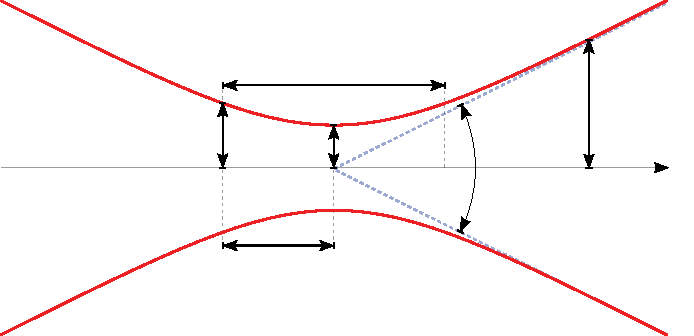
\includegraphics[width=\unitlength]{results_and_discussion/assets/GaussianBeamWaist_wiki.pdf}}%
    \put(0.20711366,0.258742){\color[rgb]{0,0,0}\makebox(0,0)[lb]{\smash{$\sqrt{2}\omega_0$}}}%
    \put(0.46945764,0.3786023){\color[rgb]{0,0,0}\makebox(0,0)[lb]{\smash{$b$}}}%
    \put(0.40642304,0.25814167){\color[rgb]{0,0,0}\makebox(0,0)[lb]{\smash{$\omega_0$}}}%
    \put(0.88008299,0.33378319){\color[rgb]{0,0,0}\makebox(0,0)[lb]{\smash{$\omega(z)$}}}%
    \put(0.97412911,0.23552655){\color[rgb]{0,0,0}\makebox(0,0)[lb]{\smash{$z$}}}%
    \put(0.7029858,0.28052652){\color[rgb]{0,0,0}\makebox(0,0)[lb]{\smash{$\vartheta$}}}%
    \put(0.38180954,0.10125008){\color[rgb]{0,0,0}\makebox(0,0)[lb]{\smash{$z_\mathrm{R}$}}}%
  \end{picture}%
\endgroup%

	\caption{The geometry of a focal region of a laser beam. The beam is
	considered to be cylindrically symmetric about the $z$ axis, the effective
	volume of the Raman sample was taken to be the volume of a cylinder of
	diameter $2\omega_0$ and length $2b$. Adopted from
	\textcite{GaussianBeamWaist}.}
	\label{\figlabel{GaussianBeamWaist_wiki}}
\end{figure}

The beam radius $\omega(z)$ can be described as the function of $z$
coordinate by equation
\begin{equation}
	\omega(z) = \omega_0\sqrt{1+\left(\frac{2z}{b}\right)^2}.
	\label{\eqnlabel{focus_optimization:beam_radius}}
\end{equation}

As a first estimation, consider non-resonance Raman scattering produced from
homogenous infinite medium and arising only from the region with the highest
illumination intensity. Furthermore, assume the loss of the illumination beam
intensity due to the Raman scattered light as negligible and that the Raman
medium is fully transparent to excitation and scattered light, it means that
there is negligible absorption and stimulated emission. The amount of Raman
scattered light from the thin transverse slice of the excitation beam is
independent of the distribution of the energy in the slice and therefore is
proportional to the total illuminating laser-beam power under these
assumptions. Then, view the Raman emission from the particular direction in
the plane of the slice. The emitted flux would be the integrated flux from
all elements on the line intersecting the slice so there would be a linear
increase of the number of elements with the increasing diameter, but each
element illumination power decreases with the square of the diameter of the
illuminating beam.

Considering the \eqnref{focus_optimization:beam_radius} derive the
approximate dependence of irradiance of that point by the Raman-scattered
light on the $z$ coordinate
\begin{equation*}
	I \propto \frac{1}{\omega(z)} \propto \frac{1}{\sqrt{1 + (2z/b)^2}}.
	\label{\eqnlabel{focus_optimization:slice_irradiance}}
\end{equation*}

So, the irradiance at $z = b$ will be reduced from the $z = 0$ by a factor of
$1/\sqrt{5} \doteq 0.447 \doteq 1/2$. For the next calculation, the brightest
region of excitation beam was approximated by the “source cylinder” of length
$2b$ and diameter $2\omega_0$ and therefore included only the brightest
region of Raman emission and neglect the emission from less-bright regions.
The source parameters are then \parencite{Barrett1968}:
\begin{align}
	\text{length:}&
		& L_\text{E}& = 16\lambda/(\text{\g{p}}\vartheta^2)
	\label{\eqnlabel{focus_optimization:L_E}}\\
	\text{diameter (width of scattering area):}&
		& W_\text{E}& = 4\lambda/(\text{\g{p}}\vartheta)
	\label{\eqnlabel{focus_optimization:W_E}}\\
	\text{volume:}&
		& V_\text{E}& = 64 \lambda^3/(\text{\g{p}}^2\vartheta^4)
	\label{\eqnlabel{focus_optimization:V_E}}\\
	\text{length-to-diameter ratio:}&
		& L_\text{E}/W_\text{E}& = 4/\vartheta.
	\label{\eqnlabel{focus_optimization:LW_E}}
\end{align}

These approximations apply to diffraction-limited Gaussian beams (
TEM\textsubscript{00}), for low-order transverse modes or combination of such
modes, the calculations based on these equations can be considered accurate
within an order of magnitude.

Many simple arguments \parencite{Atwood1963,Barrett1968} were used to propose
that the Raman spectrometer using right angle geometry scattering geometry
will gain higher signal if the laser beam is more focused. None of these
arguments, however, do not establish if there is an optimum degree of
focusing less then the largest practical value. \textcite{Barrett1968} showed
that such an optimum exists theoretically; they calculated its approximate
value, and they compared the Raman power that can be usefully collected at
that optimum degree of focusing with the total emitted Raman power.

It is known that the light is scattered to all directions by the Raman effect
and within the assumptions stated above, the Raman intensity is linearly
proportional to the excitation laser beam power. Therefore, if the amount of
Raman scattered light gathered by the spectrometer should be maximized, the
light needs to be collected from the largest solid angle and the largest
possible illuminated volume. Typical Raman spectrometer light collecting path
has two optical parts, spectrograph, and light collecting optics. Let
consider their parameters as given even though similar considerations as
bellow can also be applied to the light collecting optics optimization. Lets
further consider that the spectrograph consists of an entrance slit, imaging
optics, dispersing element, and CCD camera.

For simplicity approximate the source as flat ribbon with the same length and
width as specified above for the “source cylinder” which radiates uniformly
to all collected angles from all parts of its surface. Then, consider that
the light collecting optic displays the entrance slit of the spectrograph to
the center of the focal region of the illuminating beam. The width of the
slit $W_\mathrm{s}$ is determined by the spectrograph settings, particularly
by the desired spectral resolution, and its length $L_\mathrm{s}$ could be
estimated as an image of the CCD chip through the spectrograph. Moreover,
suppose that the aperture of light collecting optic is large enough further
not to constrain the collected Raman light over the spectrograph aperture.

Then there are two competing processes. The assumptions above that the amount
of the Raman scattered light from all thin transverse slices of the
excitation beam is the same implies that the total amount of Raman scattered
light from the source ribbon is dependent only on its length. As the focal
length of the excitation beam focusing lens is decreased, the source ribbon
is getting narrower, which results in more intensive emission of the
scattered light per unit area. So if we start with the source ribbon width
larger than the image of the spectrograph entrance slit width, the amount of
collected light increases with the narrower source ribbon. In the opposite,
the length (and therefore the total Raman scattered light intensity) of the
source ribbon decreases with the decreasing focal length of the excitation
beam focusing lens and so when the source ribbon gets shorter than the image
of the spectrograph entrance slit length, the amount of collected light
decreases with the shorter source ribbon.

So, lets split further analysis of the dependence of the Raman flux
transmitted through the spectrometer on the focusing angle of the excitation
beam $\vartheta$ (\eqnref{focus_optimization:theta}) to regions divided by
two focusing angles $\vartheta_\mathrm{W}$ and $\vartheta_\mathrm{L}$. The
$\vartheta_\mathrm{W}$ defines focusing angle at which the width of the
focusing ribbon $W_\text{E}$ is the same as the width $W$ of image of the
spectrograph entrance slit width $W_\text{S}$, and $\vartheta_\mathrm{L}$ is
angle which causes equality of the source ribbon length $L_\text{E}$ and
length $L$ of the spectrograph entrance slit image length $L_\text{S}$ on the
source. Further, define magnification of the scattered light collecting
optics as $M$. Then
\begin{align}
	L& = \frac{L_\mathrm{S}}{M}
	\label{\eqnlabel{focus_optimization:slit_length_magnification}}\\
	W& = \frac{W_\mathrm{S}}{M}
	\label{\eqnlabel{focus_optimization:slit_width_magnification}}
\end{align}
and using \eqnref{focus_optimization:L_E} and
\labelcref{\eqnlabel{focus_optimization:W_E}} and putting $L = L_\mathrm{E}$
and $W = W_\mathrm{E}$ respectively we get
\begin{align}
	\vartheta_\mathrm{W} = \frac{4\lambda}{\text{\g{p}}W}
		= \frac{4\lambda M}{\text{\g{p}}W_\mathrm{S}}
	\label{\eqnlabel{focus_optimization:theta_W}}\\
	\vartheta_\mathrm{L} = \sqrt{\frac{16\lambda}{\text{\g{p}}L}}
		= \sqrt{\frac{16\lambda M}{\text{\g{p}}L_\mathrm{S}}}.
	\label{\eqnlabel{focus_optimization:theta_L}}
\end{align}

For our spectrometer, we have $W_\mathrm{S} = 50$\,\g{m}m and beam diameter
$d = 0.9$\,mm. The wavelength can be calculated from the wavelength in vacuum
$\lambda_0 = 257.2$\,nm divided by the refractive index of water
$n_{257} = 1.3598$ \parencite{Hale1973} $\lambda = 189.1$\,nm The
$L_\mathrm{S}$ can be calculated from the height of the CCD chip
$L_\text{CCD} = 6.9$\,mm and magnification of spectrograph
$M_\text{spc} = 1.1$ as
$L_\text{S} = L_\text{CCD}/M_\text{spc} \doteq 6.3$\,mm, the magnification $M$
may be computed from focal length of objective $f_\text{o} = 13$\,mm and
focusing lens before monochromator $f \text{c} = 101.6$\,mm as
$M = f_\text{c}/f_\text{o} \doteq 7.82$. Then, from the above equations, we
calculate
\begin{align}
	\vartheta_\mathrm{W} \doteq 0.0376
	\label{\eqnlabel{focus_optimization:theta_W_calc}}\\
	\vartheta_\mathrm{L} \doteq 0.0346,
	\label{\eqnlabel{focus_optimization:theta_L_calc}}
\end{align}
which correspond regarding \eqnref{focus_optimization:theta} to
\begin{align}
	f_\mathrm{W} \doteq 24\,\text{mm}
	\label{\eqnlabel{focus_optimization:f_W_calc}}\\
	f_\mathrm{L} \doteq 26\,\text{mm}
	\label{\eqnlabel{focus_optimization:f_L_calc}}
\end{align}
respectively.

We can note, that $\vartheta_\mathrm{W}$ is greater then
$\vartheta_\mathrm{L}$, which is according to \textcite{Barrett1968} common
for the tabletop spectrometer with moderate resolution and with fairly fast
focal ration. So we can divide further analysis into three regions according
to excitation beam focusing angle
$\vartheta$: $0 \leq \vartheta < \vartheta_\text{L}$;
$\vartheta_\text{L} < \vartheta < \vartheta_\text{W}$;
$\vartheta_\text{W} < \vartheta$.

Under the approximations above the Raman flux fraction $F$, collected by the
spectrometer of the total Raman flux emitted by the source ribbon into all
angles (i.e. full solid angle of $4\text{\g{p}}$), can be estimated now. For
the simplicity, polarization effects of input and output are further ignored
and the Raman emission is assumed isotropic over all angles of collection.
Define the solid angle subtended by the spectrometer pupil as
$\Omega_\mathrm{S}$ and corresponding scattered light collecting solid angle
at the source ribbon as $\Omega$. Then
\begin{equation}
	\Omega = \Omega_\mathrm{S}M^2.
	\label{\eqnlabel{focus_optimization:omega_magnification}}
\end{equation}
For our spectrometer the solid angle of acceptance of monochromator may be
calculated from monochromator $f/\# = f/6.4$ as
$\Omega_\text{S} =
	2\text{\g{p}}\left[1 - \cos\left(\arctan\frac{1}{6.4}\right)\right]
	\doteq 0.075$\,rad.

The Raman flux fraction $F$ is then calculated from the solid angle fraction
$\Omega / 4\text{\g{p}}$ and the fraction of the light which is “masked out”
by the width of the slit image and fraction of the ribbon length as compared
to the height of the slit image using \cref{%
\eqnlabel{focus_optimization:L_E},%
\eqnlabel{focus_optimization:W_E},%
\eqnlabel{focus_optimization:slit_length_magnification},%
\eqnlabel{focus_optimization:slit_width_magnification},%
\eqnlabel{focus_optimization:omega_magnification}}.

For the first $0 \leq \vartheta < \vartheta_\text{L}$ region, the whole

slit-image width and height are illuminated, but the focused beam is wider
than slit width, and therefore the radiant flux density in the sample is
smaller (recall that we assumed that radiant losses in the sample are
negligible)
\begin{equation}
	F_\text{I}(\vartheta)
		= \frac{W}{W_\text{E}}\cdot\frac{\Omega}{4\text{\g{p}}}
		= \frac{\frac{W_\text{S}}{M}}{\frac{4\lambda}{\text{\g{p}}\vartheta}}
			\cdot\frac{\Omega_\text{S}M^2}{4\text{\g{p}}}
		=	\frac{W_\text{S}\Omega_\text{S}M}{16\lambda}\vartheta.
	\label{\eqnlabel{focus_optimization:F_I}}
\end{equation}

In the next second region
$\vartheta_\text{L} < \vartheta < \vartheta_\text{W}$,
only the whole slit-image width is illuminated, but the exciting beam is
focused to an area with smaller length than is the slit length and so the
radiant flux density is diminished by the ratio between scattering area
length and slit-image length
\begin{equation}
	F_\text{II}(\vartheta)
		= \frac{W}{W_\text{E}}\cdot\frac{\Omega}{4\text{\g{p}}}
			\cdot\frac{L_\text{E}}{L}
		=	\frac{\frac{W_\text{S}}{M}}{\frac{4\lambda}{\text{\g{p}}\vartheta}}
			\cdot\frac{\Omega_\text{S}M^2}{4\text{\g{p}}}
			\cdot\frac{\frac{16\lambda}{\text{\g{p}}\vartheta^2}}
				{\frac{L_\text{S}}{M}}
		= \frac{W_\text{S}\Omega_\text{S}M^2}{\text{\g{p}}L_\text{S}}
			\cdot\frac{1}{\vartheta}.
	\label{\eqnlabel{focus_optimization:F_II}}
\end{equation}

The Raman scattering area in the third region $\vartheta_\text{L} < \vartheta$
is so small that the Raman scattered light is collected from the whole beam,
and therefore whole radiant flux is used
\begin{equation}
	F_\text{III}(\vartheta)
		= \frac{\Omega}{4\text{\g{p}}}\cdot\frac{L_\text{E}}{L}
		= \frac{\Omega_\text{S}M^2}{4\text{\g{p}}}
			\cdot\frac{\frac{16\lambda}{\text{\g{p}}\vartheta^2}}
				{\frac{L_\text{S}}{M}}
		= \frac{4\lambda\Omega_\text{S}M^3}{\text{\g{p}}^2L_\text{S}}
			\cdot\frac{1}{\vartheta^2}.
	\label{\eqnlabel{focus_optimization:F_III}}
\end{equation}

\begin{figure}
	\centering
	\input{results_and_discussion/assets/F}
	\caption{A plot of the values of the fractional Raman flux $F$ as calculated
	for our experimental conditions using \cref{%
		\eqnlabel{focus_optimization:F_I},\eqnlabel{focus_optimization:F_II},%
		\eqnlabel{focus_optimization:F_III}}
	versus the focusing angle $\vartheta$ of the
	illuminating laser beam.}
	\label{\figlabel{focus_optimization:F}}
\end{figure}

The results of \cref{%
		\eqnlabel{focus_optimization:F_I},%
		\eqnlabel{focus_optimization:F_II},%
		\eqnlabel{focus_optimization:F_III}}

for our experimental setup can be seen in \figref{focus_optimization:F}. The
optimum value of $\vartheta$ is $\vartheta_\text{L}$. \textcite{Barrett1968}
proposed the optimum value to lie above the $\vartheta_\text{L}$ because the
signal from outside the cylinder along the excitation beam axis is also
transmitted through the spectrometer in the second and third region, but they
do not expect the optimum as high as $\vartheta_\text{W}$. The light
collecting optics magnification can be optimized according to the equations
from above too, but each equation must be multiplied by the length of the
slit image $L$. The Raman signal then does not decrease with the
magnification, which means that the magnification should be used as high as
practical.

From these considerations follows conclusion for our experimental setup, that
the optimal focal length of the laser beam focusing lens for the off-
resonance Raman spectroscopy should be somewhere between 18 and 22\,mm which
is impractically small.

All the above calculations, however, neglected loss of the excitation beam
power as it goes through the sample, but we want to use the instrument for
resonance Raman spectroscopy where significant absorption inside the sample
occurs. It can decrease the length of the source cylinder $L_E$ significantly
and can push the $\vartheta_\text{L}$ to much lower values. For example, we
typically use samples with absorbance between 5 and 50 at 257\,nm in a 1cm
cuvette. So, for example, the intensity of incident light is halved in
300\,\g{m}m path through the sample with absorbance 10 but the
$L_E = 802$\,\g{m}m at $\vartheta_\text{L}$. If we correct the
\eqnref{focus_optimization:L_E} to for example one fourth, then the
corrected $L_E,corr$ would be approximately 170\,\g{m}m and corresponding
focal length of the laser beam focusing lens about 52\,mm.

The absorbing medium brings additional complications. For example, the
anomalous refractive index near the absorption band can significantly
influence the focused beam waist, and laser beam absorption can cause local
heating which also influences refractive index and moreover produces currents
in the sample. There is also a dependence of the optimal focal length on the
excitation wavelength, but exchanges of the focusing lens in dependence on
the excitation wavelength was impractical.

However, in conclusion, the focusing lens should have the focal length as
small as possible following the experimental geometric constraints.



\subsection{Wavenumber calibration}
\begin{docitemize}
	\item Overview possibilities
	\item Describe why cyclohexane and deuterated cyclohexane
	\item Describe created calibration program
	\item Describe the advantages and disadvantages of using organic solvents
	\item Describe the possibility of use Hg lamp
	\item Describe the advantages of Pt lamp
	\item Describe parameters of the new Pt lamp
	\item Present spectrum of Pt lamp
	\item Show new schema of the apparatus
\end{docitemize}


\subsection{Polarized measurements}
\begin{docitemize}
	\item Describe tested elements
	\item Describe polarizers evaluation
\end{docitemize}


\subsection{Spinning cell}
\begin{docitemize}
	\item Overview possible solutions
	\item Draw a schema
	\item Describe the used cell
	\item Describe the method of calibration of the dependence of the rotation
	speed on the input voltage
\end{docitemize}


\subsection{Redesign for multiple excitation wavelengths}
\begin{docitemize}
	\item Draw a new spectrometer schema
	\item Describe briefly newly used elements
\end{docitemize}


\subsection{Redesign for backscattering}
\begin{docitemize}
	\item Present new schema
	\item Briefly describe new optics
	\item Present schema of mirror holder right in front of Cassegrain
\end{docitemize}


\subsection{Thermostated sample holder}
\begin{docitemize}
	\item Draw the technical drawing
	\item Present the used elements
	\item Overview the performance
\end{docitemize}
